\chapter{\uppercase{Introduction}} \label{chapter:01}

\section{Preliminaries}
Talk about the collection of noisy data, the types of inferences one may be interested in making from them.
Roughly breaks down into
\begin{itemize}
  \item Parameter Identification
  \item Distribution Estimation
\end{itemize}

Motivations break down by

\begin{itemize}
  \item Direct inference on something of interest
  \item Inference for the purpose of prediction
  \item Description of uncertainty around either of the aforementioned
\end{itemize}

\subsection{Motivations}\label{sec:motivations}
In some respects, the practice of writing software has diverged from the motivations of an academic researcher.
The latter seeks to generate new knowledge and may write a set of example scripts/programs to demonstrate some novel idea or method.
By contrast, the motivations of a software engineer are related to resiliency.
Not only must they ensure the code works as expected given a myriad of ways users may interact with it, but it is necessary to write the code in a manner compatible with maintaining it into the future.
Much of the work of writing ``good software'' is concerned with writing appropriate documentation to express the intended usage and logic underlying architectural decisions.
There are many ways to write a functioning program to demonstrate a proof-of-concept, but creating something that is \emph{user-friendly}, guaranteed to be free of mistakes, and scales across different computational environments/resources requires an entirely different approach.

Decisions made early in the software design cycle have lasting impacts on future features and functionality.
Rigor is added to libraries through the writing of \emph{unit tests}, and use of \emph{continous integration} ensures that the download and installation process is predictable and reproducible.
Code that only runs on the computer of the author is impractical since any thorough critique requires independent verification.
Without proper context and architecture, new ideas that are implemented in programs are unlikely to be adopted.

\subsection{Reproducibility}
This thesis is concerned not only with a demonstration of novel mathematical content\---showcasing new ways to make inferences from noisy data in a novel Data-Consistent framework\---it also serves to document the process of ensuring that the work herein is \textbf{fully reproducible}.
In mathematics, reproducibility is ensured through the use of proofs, which motivate the original work presented here.
However, as the title of this thesis suggests, much of the focus is actually on the computational implementation of the novel research into Data Consistent Inversion, studying the impact of using computers to perform the task of making conclusions based on data.
The implementation of mathematics on computers is done through software.
We are therefore concerned with ensuring the expected functionality of that software, which aligns with our training as mathematicians; we care deeply about making sure things are rigorous.

In short, we want to make sure that theory aligns with practice, and that both live up to high standards of intellectual scrutiny.
Every computational result, illustrative figure, table, plot, etc. presented in this thesis is associated with the scripts that generate them, and are included in the  repository for this document [TK - cite].
It is written in \LaTeX~(which is itself a programming language), and presents its own software dependencies in addition to those required to run the scripts to generate the images and tables.
To address this concern, we leverage \emph{Travis}, a continuous integration service [TK-cite], to ensure that all figures can be generated and the \LaTeX\, document compiles into a PDF.

The same care is taken to ensure the reproducibility of all numerical results based on software.
An \emph{image} that contains a fully pre-built Linux software environment within which one can compile the thesis and run the code is available through the Docker Cloud registry [TK -cite].
The latter enables the ability to generate this thesis document in its entirety on any software platform that supports Docker (Windows, MacOS, Linux).
A cloud service called Binder [ TK - cite mybinder.org] allows one-click deployments in any web-browser, removing the need for any installation whatsoever for anyone wanting to reproduce the contents of this document. 

\section{Framework}\label{sec:framework}

We provide a summary of the notation, definitions, problem-formulation, and assumptions considered in this proposal. 
For more details,  we refer the interested reader to \cite{BES12, BE13, BET+14}. 

Let $u$ be the solution to a model $\M(u, \param) = 0$, perhaps of a physical system such as the amount of contaminant in a subsurface. 
Let $\param$ represent a parameter into such a model, e.g. the permeability of the medium in the subsurface through which a contaminant is spreading.
Such parameters are often uncertain and we begin the quantification of uncertainty by identifying the set of all physically plausible parameters denoted by $\pspace\subset\RR^\dimP$.
Since different choices of $\param \in \pspace$ often lead to different model solutions, we write $u\lam$ to make this dependence explicit.

However, we cannot in general observe the entire solution $u(\param)$.
Instead, we are often limited in our ability to observe data related to some quantities of interest (QoI), defined as functionals of $u\lam$ (e.g. the contaminant levels at a specific well at a particular time).
We let $\qoi$ denote the QoI map from the solution space of the model to the space of observable data. 
Then, given $\param \in \pspace$, we obtain $u\lam$ and compute $\qoi(u\lam)$ to get the QoI datum predicted by the model.
Clearly, the QoI map depends on $\param$ through the dependency of $u$ on $\param$, so we write $\qlam$ to simplify our notation.
We assume this map is at least piece-wise differentiable.	
The data space $\dspace \subset \RR^d$ is defined as the range of the QoI map $\qoi$, i.e. 
\[
\dspace = \qoi(\pspace).
\]
In other words, we use $\dspace$ to denote the space of all physically plausible data for the QoI that the model can predict.


Let $\pborel$ and $\dborel$ denote (the Borel) $\sigma$-algebras on $\pspace$ and $\dspace$, respectively.
The map $\qoi$ between measurable spaces $(\pspace, \pborel)$ and $(\dspace, \dborel)$ is immediately measurable by the smoothness assumption. 
Then, equipping $\pspace$ and $\dspace$ with (dominating) measures $\pmeas$ and $\dmeas$, respectively, is the final ingredient for defining probability density functions (pdfs) on the measure spaces $(\pspace, \pborel, \pmeas)$ and $(\dspace, \dborel, \dmeas)$.
In practice, $\pmeas$ and $\dmeas$ are often taken to be Lebesgue volume measures when $\pspace$ and $\dspace$ are finite-dimensional~\cite{BET+14, BJW18}.
In general, these measure allow for the description of probability measures as probability density functions defined by Radon-Nikodym derivatives.


\subsection{Problem Formulation and Solution}

We begin with defining the types of forward and inverse problems considered in this thesis.

\begin{defn}[Forward Problem]\label{defn:forward-problem}
  Given a probability measure $\PP_\pspace$ on $(\pspace, \pborel)$, and (at least piecewise-differentiable) QoI map $\qoi$, the \emph{forward problem} is to characterize a measure $\PP_\dspace$ on $(\dspace, \dborel)$ (recalling $\dspace = \qoi(\pspace)$) that satisfies
  \begin{equation}\label{eq:forward-problem}
    \PP_\dspace (E) = \PP_\pspace \left ( \qoi^{-1}(E) \right ), \; \forall \; E \in \dborel.
  \end{equation}
\end{defn}

\begin{defn}[Inverse Problem]\label{defn:inverse-problem}
  Given a probability measure $\observedP$ on $(\dspace, \dborel)$ that is absolutely continuous with respect to volume measure $\dmeas$, the \emph{inverse problem} is to determine a probability measure $\PP_\pspace$ on $(\pspace, \pborel)$, absolutely continuous with respect to $\pmeas$, satisfying

  \begin{equation}\label{eq:inverse-problem}
    \PP_\pspace (\qoi^{-1}(E)) = \int_{\qoi^{-1}(E)} \pp_\pspace \lam \, d\pmeas = \int_E \observed \q \, d\dmeas = \observedP(E), \; \forall \; E \in \mathcal{B}_\dspace.
  \end{equation} 

  \noindent Here,
   
  \begin{equation*}
    \pp_\pspace := \frac{d\PP_\pspace}{d\pmeas} \;\text{ and }\; \observed := \frac{d\observedP}{d\dmeas}
  \end{equation*}
  denote the Radon-Nikodym derivatives (i.e., pdfs) of $\updatedP$ and $\observedP$, respectively. 
  Any probability measure $\PP_\pspace$ satisfying \eqref{eq:inverse-problem} is referred to as a \emph{consistent solution} to the inverse problem, and \eqref{eq:inverse-problem} is referred to as the \emph{consistency condition}.
\end{defn}

In measure-theoretic terms, $\updatedP$ is a pull-back measure of $\observed$.
From the perspective of a forward problem, we seek $\updatedP$ such that its push-forward measure is equivalent to $\observed$. 
In other words, the solution we seek to the inverse problem is constrained by a forward problem. 
Below, we formalize some of the vocabulary involved in the formulation and solution of the stochastic inverse problem.

\begin{defn}[Observed Distribution]\label{defn:observed}
  The density $\observed$ in \eqref{eq:inverse-problem} represents the uncertainty in QoI data and is referred to as the \emph{observed distribution} (or density), and is the Radon-Nikodym derivative of the \emph{observed measure} $\observedP$ with respect to the volume measure $\dmeas$.
\end{defn}

The map $\qoi$ impacts the structure of the update since the underlying data space $\dspace$ itself depends on $\qoi$, and both densities on $(\dspace, \dborel)$ are evaluated at $\qlam$.
In the event that the map $\qoi$ is a bijection, then the consistency condition \eqref{eq:inverse-problem} defines a unique measure $\PP$ on $\pspace$ given the specification of an observed density.
However, there are many applications of interest where $\qoi$ fails to be a bijection, either due to differences in the dimensions of the parameter and data spaces, nonlinearities inherent in the model itself, or both. 


The specific nuances of this relationship are discussed in \ref{chapter:02} and \ref{chapter:03} in greater detail.
Here, we simply note that the construction of \eqref{eq:update} requires only the forward-problem construction of $\predicted$, since $\initial$ and $\observed$ are given \emph{a priori}.
Additional properties are given in \ref{sec:properties} alongside the conditions for the existence and uniqueness of an update of the form given by \eqref{eq:inverse-problem}. 



\subsection{Properties and Assumptions of Consistent Update}\label{sec:properties}

To construct a solution $\updatedP$ satisfying \eqref{eq:inverse-problem}, we adopt a Bayesian perspective of combining prior beliefs with data.

\begin{defn}[Initial Distribution]\label{defn:initial}
  The density $\initial$ is used to represent any prior beliefs about parameters before observations on QoI taken into account, and is referred to as the \emph{initial distribution} (or density).
  It can also be given as a measure $\initialP$, in which case $\initial$ is the Radon-Nikodym derivative of $\initialP$ with respect to the given volume measure $\pmeas$.
\end{defn}

To construct $\updated$, we ``push-forward'' the prior (initial) beliefs using the QoI map to compare to the evidence provided by $\observed$.
In other words, we first solve the forward problem of \eqref{defn:forward-problem} to construct a solution to the inverse problem.
To make this precise, we use the following:

\begin{defn}[Predicted Distribution]\label{defn:predicted}
  The push-forward density of $\initial$ under the map $\qoi$ is denoted as $\predicted$, and is referred to as the \emph{predicted distribution} (or density).
  It is given as the Radon-Nikodym derivative (with respect to $\dmeas$) of the push-forward probability measure \eqref{eq:forward-problem} given by
  \begin{equation}\label{eq:predicted}
    \predictedP (E) = \initialP \left ( \qoi^{-1}(E) \right ), \; \forall \; E \in \dborel,
  \end{equation}
  which should be recognizable from the definition of the forward problem.
  In other words, $\predictedP$ is the solution to the push-forward problem given $\initialP$.
\end{defn}


The stochastic inverse problem is defined as finding a measure $\PP_\pspace$ such that the push-forward of it matched $\observedP$.
The following assumption guarantees a solution to the stochastic inverse problem.
It implies that any event which is assigned a positive probability by the observations must also be assigned a positive probability of occurring by the initial beliefs.

\begin{assumption}[Predictability Assumption]\label{as:pred}
  The measure associated with $\observed$ is absolutely continuous with respect to the measure associated with $\observed$.
\end{assumption}

If this is unsatisfied, one source of information (the data) suggests certain events are probable while another source of information (the model and initial) have a priori ruled that almost surely these events should not occur.
Therefore, either initial beliefs, the model under consideration, or the description of uncertainty encoded in $\predicted$ should be subjected to a critical reevaluation.


The requirement given in Assumption~\ref{as:pred} is guaranteed if the following is satisfied:
\begin{equation}\label{eq:pred}
  \exists \; C>0 \text{ such that } \observed (d) \leq C \predicted(d) \text{ for a.e. } d\in \dspace,
\end{equation}
where it is understood that $d = \qlam$ for some $\param \in \pspace$.
Now, assuming \eqref{eq:pred} holds, we restate the following theorem from \cite{BJW18} based upon the disintegration of measures:


\begin{thm}[Existence and Uniqueness]
  For any set $A\in \pborel$, the solution $\updatedP$ given defined by
  \begin{equation}\label{eq:dci_sol}
    \updatedP (A) = \int_\dspace \left (  \int_{\pspace \in \qoi^{-1}(d)}  \initial\lam \frac{\observed\q}{\predicted\q} \, d\mu_{\pspace, d} \lam \right ) \, d\dmeas(d), \; \forall \; A \in \pborel
  \end{equation}
  is a consistent solution to the stochastic inverse problem given in (\ref{eq:inverse-problem}), and is uniquely defined up to the specification of a prior (initial) probability measure $P_\pspace$ on $(\pspace, \pborel)$.
  Here, $\mu_{\pspace, d}$ denotes the disintegration of the dominating measure $\mu_\pspace$.
\end{thm}

The updated density \eqref{eq:update} in the iterated integral in \eqref{eq:dci_sol} has no normalization constant because it is in fact a density (i.e., it integrates to $1$), which is summarized in Corollary 3.1 in \cite{BJW18} and restated in simplified form below:
\begin{cor}\label{cor:int}
$\updatedP(\pspace) = 1$.
\end{cor}

These definitions are combined to form the \emph{updated density}, originally derived in \cite{BJW18}:

\begin{defn}[Updated Distribution]\label{defn:updated}
  A solution satisfying \eqref{eq:dci_sol} is referred to as an updated distribution, with an updated density given by the Radon-Nikodym derivative,
  \begin{equation}\label{eq:update}
    \updated \lam = \initial \lam \frac{\observed \q }{\predicted \q }, \; \forall \; \param \in \pspace.
  \end{equation}
\end{defn}

Corollary~\ref{cor:int} is critical to understanding some significant differences between the statistical Bayesian updated density~\cite{Smith} and the updated density density given by \eqref{eq:update}, which we discuss in Section~\ref{sec:othermethods}.
Moreover, this Corollary provides the basis for a useful numerical diagnostic that informs us about the quality of a solution based on finite sampling and density estimation.

%%%%%%%%%%%%%%%%%%%%%%%%


\subsection{Stability of the Consistent Solution}\label{sec:stability}

We first recall the Total Variation (TV) metric on the space of probability measures, defined as
\begin{equation}\label{eq:tv}
d_{\text{TV}} (\PP_f, \PP_g) := \int \abs{f - g} \, d\mu,
\end{equation}
where $f,g$ are the densities (Radon-Nikodym derivatives with respect to $\mu$) associated with measures $\PP_f, \PP_g$, respectively.
The stability results below are all with respect to the TV metric, which is widely used in the literature and is also known as \emph{statistical distance}~\cite{GS02, Smith, Silverman}.
We first define stability with respect to perturbations in the data.

\begin{defn}[Stability of Updated Densities I]\label{defn:stableobs}
  Given $\initialP$ and $\observedP$, let $\widehat{\observedP}$ be any perturbation to $\observedP$ on $(\dspace, \dborel)$ satisfying \eqref{eq:pred}.
  Let $\updatedP$ and $\widehat{\updatedP}$ denote the consistent solutions associated with $\observedP$ and $\widehat{\observedP}$, respectively.
  We say that $\updatedP$ is \emph{stable} with respect to perturbations in $\observedP$ if for all $\eps > 0$, there exists a $\delta > 0$ such that
  \begin{equation}
    d_{\text{TV}} (\observedP, \widehat{\observedP}) < \delta \implies d_{\text{TV}} (\updatedP, \widehat{\updatedP}) < \eps.
  \end{equation}
\end{defn}

In \cite{BJW18}, it is shown that $d_{\text{TV}} (\widehat{\updatedP}, \updatedP) = d_{\text{TV}} (\widehat{\observedP}, \observedP)$, which immediately proves the following:

\begin{thm}
  $\updatedP$ is stable with respect to perturbations to $\observedP$.
  \label{thm:stableobs}
\end{thm}

This next definition and result are useful in analyzing the sensitivity of the updated density with respect to the initial beliefs.

\begin{defn}[Stability of Updated Densities II]\label{defn:stableinitial}
  Given $\initialP$ and $\observedP$, let $\widehat{\initialP}$ be any perturbation to $\initialP$ on $(\pspace, \pborel)$ satisfying \eqref{eq:pred}.
  Let $\updatedP$ and $\widehat{\updatedP}$ denote the consistent solutions associated with $\observedP$ and $\widehat{\observedP}$, respectively.
  Let $\sett{\PP_{\pspace, d}}{d\in\dspace}{}$ and $\sett{\widehat{\PP_{\pspace, d}}}{d\in\dspace}{}$ be the conditional probabilities defined by the disintegration of $\initialP$ and $\widehat{\initialP}$, respectively.
  We say that $\updatedP$ is \emph{stable} with respect to perturbations in $\initialP$ if for all $\eps > 0$, there exists a $\delta > 0$ such that for almost every $d\in\supp(\observedP)$,
  \begin{equation}\label{eq:stableinitial}
    d_{\text{TV}} (\PP_{\pspace, d}, \widehat{\PP_{\pspace, d}}) < \delta \implies d_{\text{TV}} (\updatedP, \widehat{\updatedP}) < \eps.
  \end{equation}
\end{defn}

\begin{thm}
  $\updatedP$ is stable with respect to perturbations to $\initialP$
  \label{thm:stableinitial}
\end{thm}

Taken together, these stability results provide assurances that the updated density we obtain is ``accurate'' up to the level of experimental error polluting $\observedP$ and error in incorrectly specifying prior assumptions using $\initialP$.
Given that specifying the definition of a ``true'' initial density is somewhat nebulous, we are less interested in the consequences of the latter conclusion.
However, generating samples from $\updatedP$ requires a numerical approximation to $\predictedP$, which introduces additional errors in $\updatedP$.
If $\widehat{\predicted}$ denotes a computational approximation to the push-forward of the initial density obtained with $\widehat{\predicted}$ substituted for $\predicted$ in \eqref{eq:dci_sol}, then the conditional densities from the Disintegration Theorem are given as
\[
\frac{\widehat{d\PP_{\pspace, d}}}{d\mu_{\pspace, d}\lam} = \frac{\initial\lam}{ \widehat{\predicted\q} },
\]
where $\widehat{\PP_{\pspace, d}}$ denotes the disintegration of $\widehat{\updatedP}$.
In Section~\ref{sec:approx}, the TV metric is used to bound the error in the updated density in terms of the error in the approximation to the push-forward of the initial.



%%%%%%%%% Section 2.3
\subsection{Numerical Approximation and Sampling}\label{sec:approx}
%Since we are given $\initial$ and $\observed$, the computation of $\predicted$ is the only aspect of the Consistent Bayesian framework that needs to be approximated.
%Since there are few restrictions on the structure of the map $\qoi$ that defines $\predicted$, there is in general no explicit expression from which we can generate samples, so we use a numerical approximation to the probability density function.
%
%For simplicity, we simply propagate Monte-Carlo samples from the prior and use a kernel density estimate (usually Gaussian\footnote{In this proposal, all results are generated using this kernel, though six kernels common to density estimation are implemented in the ConsistentBayes Python package [TK - cite Silverman and your github].}).
%
%We summarize this in the following algorithm:
%
%\begin{algorithm}[hbtp]
%\DontPrintSemicolon
%Generate a set of samples $\sett{\param_i}{i=1}{N}$
%	\For{$i = 1, \hdots, N$}{
%			Propagate sample $\param_i$ through the QoI map. Set $d_i = \qoi(\param_i)$.
%	}
%Use $\sett{d_i}{i=1}{N}$ and a density estimation method to approximate $\predicted$.
%	\label{alg:sample}
%\caption{Numerical Approximation of the Push-forward of the Prior Density}
%\end{algorithm}
%


%The computational object associated with $\predicted$ is stored for re-use and can be evaluated at locations in $\dspace$ other than $\sett{d_i}{i=1}{N}$.
%This procedure should be thought of as a characterization of the data space given the prior assumptions encoded in $\initial$.


Using the previous notation, we let $\widehat{\predicted(d)}$ be a computational approximation to $\predicted$ and $\widehat{\updated}$ the associated approximate updated density $\updated$.
As before, we assume the following for the approximation of the push-forward of the initial density:
\begin{assumption}\label{as:predx}
There exists some $C>0$ such that
\[
\observed (d) \leq C \widehat{\predicted(d)} \text{ for a.e. } d\in \dspace.
\]
\end{assumption}

If this assumption is satisfied, we have the following theorem from \cite{BJW18}:
\begin{thm}
  The error in the approximate updated density is bounded above:
  \begin{equation}\label{eq:predicted_bound}
    d_{\text{TV}} (\updatedP, \widehat{\updatedP}) \leq C d_{\text{TV}} (\predictedP, \widehat{\predictedP}),
  \end{equation}
  where the $C$ is the constant taken from Assumption \ref{as:predx}.
\end{thm}

In practice, we perform a forward propagation of samples from $\pspace$ to $\dspace$ and compute an approximation of $\predicted$ using density estimation~\cite{BJW18}.
Then, we may evaluate $\updated$ directly for any sample of $\pspace$ at the cost of one model solve for any sample other than the ones already propagated to approximate $\predicted$.
We leverage the re-use of samples in the results herein extensively.

In summary, the \textbf{accuracy of the computed updated density relies on the accuracy of the approximation of the push-forward of the initial.}
Throughout this proposal, we utilize a Gaussian (KDE), which converges at a rate of $\mathcal{O}(N^{-4/(4+d)})$ in mean-squared error and $\mathcal{O}(N^{-2/(4+d)})$ in $L^1$-error, where $d$ is the dimension of $\dspace$, and $N$ is the number of samples from $\initial$ propagated through $\qoi$ [TK - references for convergence rates].

%For simplicity, we introduce the following notation to capture the role of the ratio involved in \eqref{eq:dci_sol} to demonstrate properties we can leverage for generating samples from $\updated$.
%We let
%\[
%\updated\lam = \initial \lam r\q, \text{ where } r\q = \frac{\observed\q}{\predicted\q}
%\]
%
%Many standard calculations about the updated density involve integrals of functions of $r\q$ with respect to the prior.
%For any measurable function $f$, we establish the connection of calculating quantities over $\pspace$ with those over $\dspace$ by leveraging the following identity from measure theory:
%\[
%\int_\pspace f\left( r\q \right ) \, d\initialP = \int_\dspace f\left( r(d) \right ) \, d\predictedP
%\]
%
%We use several throughout this proposal, including the integral of the updated density:
%\[
%I(\updated ) = \int_\pspace r\q \, d\initialP = \int_\dspace r(d) \, d\predictedP ,
%\]
%which we can use to validate that $I(\updated) \approx 1$ in order to numerically validate that the assumption given in \eqref{eq:predicted_bound} was not violated.
%
%Similarly, we follow \cite{BJW18} to write the commonly used metric for Information Gain, the Kullback-Liebler (KL) divergence:
%\begin{equation}\label{eq:KLdiv}
%\text{KL}(\initial : \updated ) = \int_\pspace r\q \log r\q \, d\initialP = \text{KL}(\observed : \predicted ),
%\end{equation}
%i.e., the KL-divergence between the prior and updated density is equal to the KL-divergence between the observed density and the push-forward of the prior.


Where possible, we express $\predicted$ analytically for purposes of demonstration (especially for comparing numerical solutions to the exact solutions).


%%%%%%%%% Section 2.4
\subsection{Comparison to Other Methods}\label{sec:othermethods}
We establish two comparisons: first to Bayesian inversion \cite{Walpole, Berger, Complete, Smith}, the second to a measure-theoretic approach studied in \cite{BET+14, BE13}.


\subsubsection{Statistical Bayesian Approach}

%If the quantity of interest is a single measurement, then the likelihoods and observed densities are identical.
%However, the quantity of interest may not necessarily just be the uncertainty in the measurement data, as we will see in later discussions.
%For completeness, we define the alternative solution to the SIP below and compare the two frameworks under a simple linear map.

The Bayesian formulation gives a posterior density as:

\begin{equation}\label{eq:sb_post}
    \pp\lam := \initial\lam \frac{L_\dspace (d | \param)}{ C },
\end{equation}

where we use $\pp$ to distinguish the \emph{posterior} from the updated density $\updated$ in \eqref{eq:update}.

Here, we borrow the notation $\initial$ to represent the Bayesian $\pp_\text{prior}$, since in our comparative examples we use the two interchangeably.
We choose them to represent the set of feasible parameters, and rely on Monte-Carlo sampling for both approaches\footnote{Priors in Bayesian inference are sometimes chosen for reasons related to Markov-Chain Monte-Carlo algorithms in order to ensure their balancing of investigation and exploration, or convergence [TK - cite someone]}.
We compare the Bayesian posterior to our updated density, but temporarily abuse notation for the sake of comparison and use $\updated$ to refer to both, with $\pp$ representing the posterior when the distinction needs to be made.

$L_\dspace$ is the likelihood function as a function of the output and the denominator $C$ is a normalizing constant (known as the \emph{evidence} \cite{Smith}), which ensures the posterior density integrates to one:
\[
C = \int_\pspace \initial\lam L_\dspace(d | \param) \, d\param.
\]

Note that there are no constraints or requirements that likelihood function be a density\footnote{It is just the case that in order to pose problems where we can align the two methods, we need to form $L$ as a density.}.
In fact, $L_\dspace$ need not even be in $L^1(\pspace)$ since it is actually only the product $\initial(\param) L_\dspace (d | \param)$ that is required to be in $L^1(\pspace)$ to form a posterior.
In other words, $L_\dspace (d | \param)$ and $\observed(\qlam)$ can model completely different things with respect to uncertainty in the data.
An interpretation of $L_\dspace (d | \param)$ is the relative likelihood that a single parameter $\param\in\pspace$ explains the observed data, whereas $\observed(\qlam)$ describes the relative likelihood of a predicted datum associated with $\param\in\pspace$.

In this framework, there is a different notion of consistency, referring to certain asymptotic properties of $\updated$ in the limit of infinite data \cite{Barron, Silverman}.
It is important to note that the Bayesian framework poses a different question for which a different answer is sought, which is based on the presence of $L_\dspace(d | \param)$ in place of $\observed(\qlam)$.
Specifically, the problem analyzed by the Bayesian approach is to determine a single ``true'' parameter that explains all of the observed data \cite{Smith, Concrete, Complete}.
The philosophical underpinnings of Bayesian inference is akin to the asking following:

\begin{center}
  \emph{How does one incorporate collected data to shift prior beliefs about parameter values?}
\end{center}

The philosophical underpinnings of Bayesian inference are distinct from the Data-Consistent framework, where we seek a pull-back measure: a description of the uncertainty set that explains the variation in the observations under a given description of error.
This approach expresses a desire to reconstruct a distribution (or probability measure), asking:

\begin{center}
  \emph{How does one update prior beliefs in such a way that modifies predictions to match the description of uncertainty in observed data?}
\end{center}

We note that there are problems that one can formulate where the observed density corresponds directly to a normalized likelihood function familiar to Bayesian statisticians, as we demonstrate below.
One difference between the two solutions is the use of normalizing constant $C$ in $\pp$ not present in $\updated$, as discussed in Corollary~\ref{cor:int} above.
To illustrate the two approaches, we explore the impact of this difference in the example below, taken from \cite{BJW18}.

\begin{ex}
Consider
\begin{equation}
u(\param) = \param^p
\end{equation}
for $p$ chosen as either 1 or 5.
For both approaches, the prior or initial density is given by $\initial \sim U[-1,1]$.
In the Data-Consistent Inversion framework, $\observed \sim \mathcal{N}(0.25,0.1^2)$.
In the statistical Bayesian framework, we take $d=0.25$ and assume an additive error noise model with distribution $\mathcal{N}(0,0.1^2)$ so that the likelihood, $L_\dspace(d | \param)$, matches the observed density as a function of $\param$.

When $p=1$, we have $\predicted = \frac{1}{2} = C$.
Since $\observed\q = L_\dspace(d|\param)$ and $\predicted$ agrees with the normalizing constant $C$, the posterior and update agree on $\pspace$ (we show the push-forwards in the right plot of Figure~\ref{fig:comparison}).
When $p=5$, the non-linearity of the model causes the push-forward of $\initial$ to be non-constant, so the two approaches now yield differing solutions, as seen in the left plot of Figure~\ref{fig:comparison}).
The push-forward of the posterior associated with the statistical Bayesian framework is influenced by the push-forward of the prior in a way that the push-forward of the updated density avoids.

\begin{figure}
\begin{minipage}{.45\textwidth}
		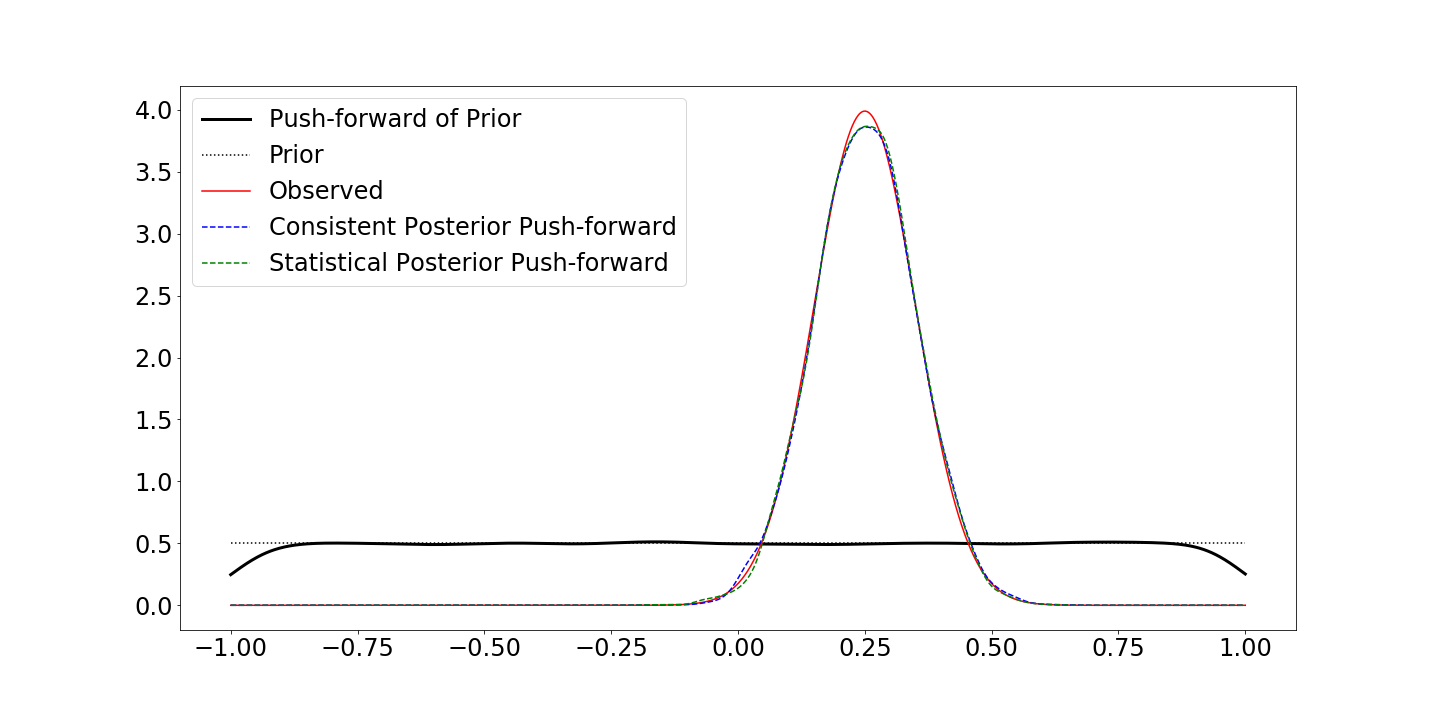
\includegraphics[width=\linewidth]{./images/comparison1}
\end{minipage}
\begin{minipage}{.45\textwidth}
		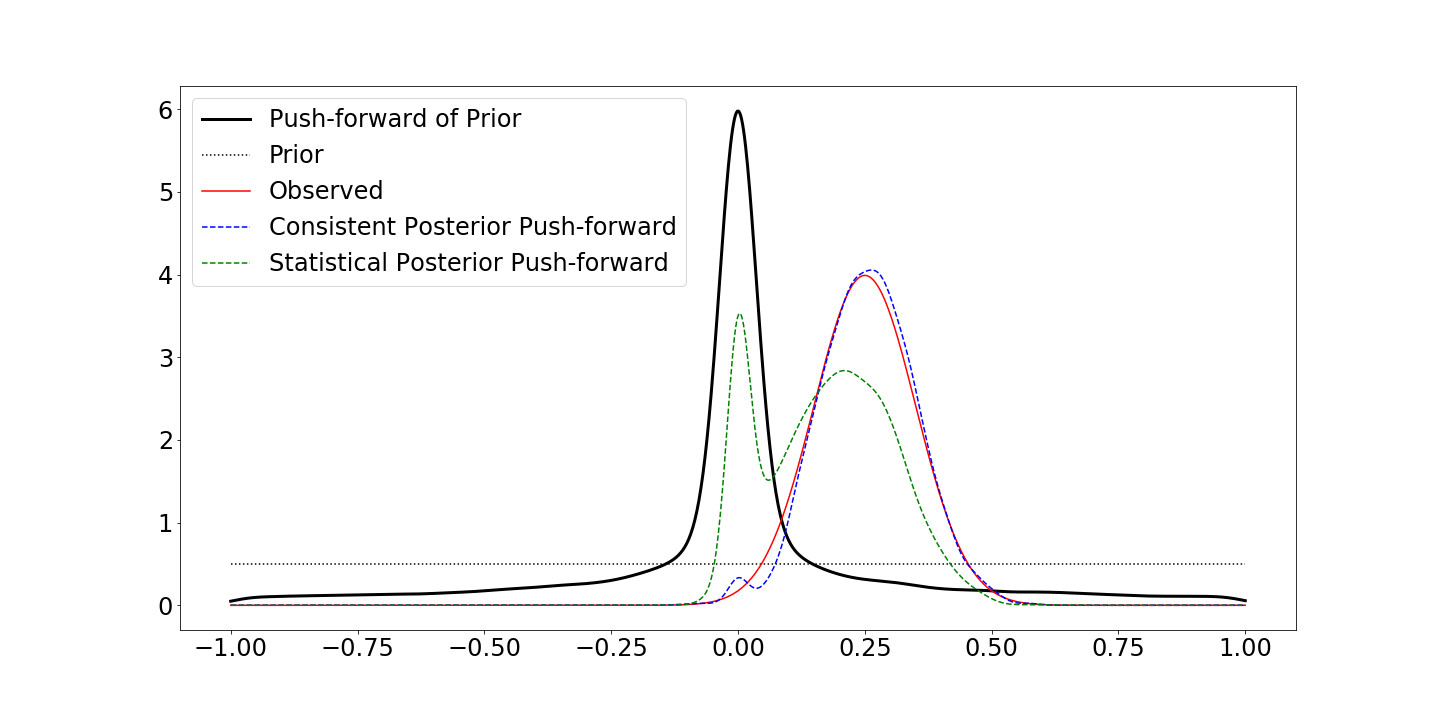
\includegraphics[width=\linewidth]{./images/comparison5}
\end{minipage}
\caption{
In each plot, the black dotted line represents the prior (initial), while the solid line represents the push-forward.
The push-forwards of the posterior (updated) densities are shown as a green (blue) dotted line.
The likelihood (observed density) is shown as a solid red line.
(Left): $p = 1$, the push-forwards of the solutions are identical because a linear map results in a constant push-forward of a uniform prior.
(Right): $p = 5$, the non-linearity of the map causes the solutions to be different and thus the push-forwards to also be different.
}
\label{fig:comparison}
\end{figure}

% [TK - removed paragraph] We can see in Figure~\ref{fig:comparison} that the two approaches pose different questions and thus yield different results.
% The Data-Consistent Inversion framework seeks to recreate the observed density, which it does for both $p=1$ and $p=5$, but the Bayesian approach is a combination of both the observed and the push-forward of the prior.
[TK - a lot of this discussion is well-covered in the intro to the mud paper... let's move it here??]
Bayesians do not push-forward their posterior density, so in some sense this comparison is not entirely fair.
It is not the goal of Bayesian inference to recreate the likelihood function in this way.
Rather, the point of maximum likelihood would be propagated and perturbed with the assumed noise model.
This is because Bayesian inverse problems are fundamentally posed as parameter-identification (an optimization to be performed), not distribution estimation.
In the event that a Bayesian would want to estimate a distribution, they would do so by creating a parametric representation thereof.
For example, one could assume that a posterior on $\pspace$ can be expressed as a Gaussian distribution, and solve for the most likely mean and standard deviation that characterizes it [TK - cite more] \cite{Smith}.
Nonparametric densities can be approximated by mixture models.
For example, one can assume that the posterior can be given by a linear combination of four Gaussian distributions, and solve for eight parameter values (four standard deviations and means).
However, the operative word here is \emph{assume}; in order to capture a density using a Bayesian framework, one needs to impose some sort of explicit structure on the posterior.
No such compromise is required in the Data-Consistent Inversion framework.
Distributions (or measures) can be solved for directly, regardless of any nonlinear/non-parameteric structure by leveraging the measure-theoretic approach described in \cite{BE13} or \cite{BJW18}.

\end{ex}



\section{Software Contributions}\label{sec:ch01-software}

As discussed in \ref{sec:motivations}, the entirety of the mathematical content herein has been incorporated into freely available open-source software, including this work itself.
The novel mathematical developments that have gone into the work herein are all reflected in various modules and sub-modules as part of the BET Python package.
This software suite follows a number of industry best-practices for code-coverage (\ref{sec:code-coverage}) and continuous integration (\ref{sec:continuous-integration}), i.e. the code is well-tested (\ref{sec:unit-testing}).

A significant proportion of the effort involved in the writing of this thesis revolved around learning about the art and practice of modern (open-source) software development.
As new ideas sprang up, our research group found itself coding and re-coding the same methods that had yet to be incorporated into user-friendly, computationally efficient, and properly-parallelized libraries.
Over the years, the software fell behind the state-of-the-art in research, and previous maintainers of code had moved on from their academic positions.
The author spent most of 2019 bringing the software in-line with the latest developments in Data-Consistent Inversion.


\subsection{Software Design and Architecture}\label{sec:architecture}

Having learned a lot about software reproducibility along the way, the author made the decision to treat this thesis as a software project in its own right.
Every example, figure, table, and plot is generated by a combination of Python and Bash scripts contained inside of a public Github repository (www.github.com/mathematicalmichael/thesis).

By hosting this work on Github, corrections can be submitted as Issues, and the document can serve as a reference point for a thorough introduction on the topic of Data-Consistent Inversion.
All the requisite \LaTeX~dependencies are contained in {\tt apt.txt}, and a Jupyterlab environment usable by Binder (which can compile the document and run every example) is configured in the {\tt binder/} directory of the repository (on the binder branch).

Special care is taken to ensure that every file herein is well-documented.
When appropriate, functions and classes are used in such a way that the same file generates several examples generated.
The parameters required are passed as optional arguments, and bash scripts containing the exact syntax to generate each figure are included.

For example, to visually demonstrate the implicitly-defined sets of nearest-neighbors in two-dimensional unit domain, we rely on Voronoi-cell diagrams.
One python file (\bashinline{images/voronoi_unit_domain.py}) contains the methods required to draw a single figure/illustration.
Some plots require labels, and others do not, and at one point we demonstrate the impact of random sampling on the geometry of the induced computational equivalent of a $\sa$.
To accommodate the need for different variations of similar plots, we utilize the argument-parsing package \pythoninline{argparse}, part of the Python standard library, to enable command-line positional and optional arguments \footnote{We equip each function with default values so that the syntax \bashinline{python example.py} without any additional arguments will work, but specific examples rely on optional arguments to be passed accordingly.}.
We include associated (wrapper) files with descriptive names, such as \bashinline{images/make_voronoi_diagrams.sh} that repeatedly call the relevant python file(s) and passes arguments (such as {\tt num} for ``number of samples'').
We refer the inquisitive reader to  Figure~\ref{fig:voronoi_cells} or \ref{fig:voronoi_issues} to see the Voronoi-cell diagrams generated by the following script\footnote{A \LaTeX macro has been written to allow for Python and Bash files to be displayed contextually to avoid the need to update them in two places. What is shown here is exactly what gets run. When scripts are long, important sections of code may be interspersed within the text, with the full script available in the appendix associated with the chapter.}:

\bashexternal{images/make_voronoi_diagrams.sh}


These wrappers are called by other Bash scripts which are each responsible for generating figures in different sections or specific models (QoI maps).
This builds something akin to a ``tool chain,'' a series of calls to hierarchies of scripts in order to generate the pictorial content in this work.


\subsubsection{Continuous Integration}\label{sec:continuous-integration}

These outer-level scripts that call others are leveraged by \emph{Travis}, a continuous-integration (CI) service that runs a series of commands on behalf of the user, automating the process of testing functionality.
The familiarity with this technology was introduced as a consequence of working on BET \cite{pyBET}, the software library that originally implemented the set-based approach discussed in \ref{sec:ch02-set}.
The use of CI in BET is similar to that of most software packages written in Python, unit tests are run in some framework (\pythoninline{nose} for BET, alternatively \pythoninline{pytest}), and a successful run triggers a webhook that communicates with the software repository host (Github) to validate changes.

\subsubsection{Testing}\label{sec:unit-testing}
The aforementioned \emph{unit tests} are a framework for guaranteeing the behavior of programs or individual methods when instructions are followed.
\emph{Functional tests} encompass more complicated behavior, stringing together several methods/modules to ensure code runs as its author intended, and are usually included when referring to unit testing.
``How to write a test'' is a question that depends highly on the particular functionality, but the premise is always the same.

[TK - maybe show a really basic example of a set/get method and the test for that?]


\subsubsection{Code Coverage}\label{sec:code-coverage}

Code coverage refers to the proportion of lines of code that were run during the process of testing (consisting of unit and functional tests).
The goal is not necessarily to achieve 100\% coverage, but rather to make sure that the most crucial use-cases are checked.
Generally speaking, coverage in the 75-85\% range is industry-standard.

[TK - flesh out a bit more, talk about Codecov, the specific service we use, how it won't be used for the scripts in this thesis].


\subsubsection{BET Architecture}\label{sec:bet-architecture-overview}

The fundamental class in the BET implementation of Data-Consistent Inversion is the \pythoninline{discretization} object, which holds the representation of an inverse problem.

The parameter space $\pspace$ is represented as an \pythoninline{input_sample_set} attribute to the \pythoninline{discretization} instance.
Similarly, $\dspace$ is associated with a \pythoninline{output_sample_set}.
The measure/density $\observedP$ (or $\PP_\dspace$) that is imposed on $\Dspace$ is held as an \pythoninline{output_probability_set} attribute.
Each of these is an instance of a \pythoninline{bet.sample_set} class.

[TK - talk about a few of the core properties of these classes, but perhaps save the diagrams for Ch2].
More details will follow in \ref{sec:ch02-software}, as is an overview of the development timeline.
